% Copyright (C) 2001-2019 Peter Selinger.
% This file is part of Potrace. It is licensed under the GNU General
% Public License. See the file COPYING for details.

\documentclass{article}
\usepackage{times}
\usepackage{graphics}

\title{Potrace Library API}
\author{}
\date{}

% Alphabetic labels
{\makeatletter
\gdef\alphalabels{\def\theenumi{\@alph\c@enumi}\def\labelenumi{(\theenumi)}}}

\begin{document}
\maketitle

\noindent {\it Copyright \copyright\ 2001-2019 Peter Selinger.  
  This file is part of Potrace. It is licensed under the GNU General
  Public License. See the file COPYING for details. }

\section{Scope}

The Potrace library provides:

\begin{itemize}
\item tracing, i.e., conversion of bitmaps to a vector representation
  (Bezier curves and straight line segments).
\end{itemize}
It does not provide frontend functionality such as:

\begin{itemize}
\item preparation of bitmaps (e.g.\ reading a bitmap from a file, preparing
  a bitmap by thresholding/scaling/filtering a greyscale image etc)
\end{itemize}
And it does not provide backend functionality such as:

\begin{itemize}
\item post-processing of the vector representation (e.g.\ conversion to a
  file format such as PostScript or SVG, scaling + rotation,
  quantization etc).
\end{itemize}

\section{Data representation}

\subsection{Bitmaps}\label{ssec-bitmap}

\subsubsection{Coordinate system}

\begin{figure}[t]
\[ \includegraphics*[0in,0in][3in,1.7in]{potracelib-fig3}
\]
\caption{The Potrace coordinate system}\label{fig-coord}
\end{figure}

For Potrace, a bitmap of size $w\times h$ is embedded in a cartesian
coordinate system where each pixel takes up the space of one unit
square. The pixels are positioned so that the {\em corners} of pixels
(and not their centers) lie at points with integer coordinates, as
illustrated in Figure~\ref{fig-coord}. The origin of the coordinate
system is at the {\em lower left} corner of the bitmap. The four
corners of the bitmaps have coordinates $(0,0)$, $(0,h)$, $(w,h)$, and
$(w,0)$.

Sometimes we need to refer to a specific pixel (as opposed to a point
in the plane). When we speak of ``pixel $[i,j]$'', we mean the pixel
whose corners have coordinates $(i,j)$, $(i,j+1)$, $(i+1,j+1)$,
$(i+1,j)$ in Potrace's coordinate system. Thus, pixel $[i,j]$ is the
pixel whose center is at coordinates $(i+0.5, j+0.5)$. To avoid
confusion, we use square brackets to refer to the pixel $[i,j]$, and
round brackets to refer to the point $(i,j)$.

\subsubsection{Bitmap representation}

The Potrace library expects bitmaps in the following format, defined
in potracelib.h:

\begin{verbatim}
struct potrace_bitmap_s {
  int w, h;          /* width and height, in pixels */
  int dy;            /* scanline offset in words */
  potrace_word *map; /* pixel data, dy*h words */
};
typedef struct potrace_bitmap_s potrace_bitmap_t;
\end{verbatim}

Here, \verb!potrace_word! is an unsigned integer type defined in
potracelib.h. It is usually equal to a native machine word (i.e., 32
bits on a 32-bit architecture). In the following explanation, we
assume that the type \verb!potrace_word! holds $N$ bits.

A bitmap of dimensions $w\times h$ is divided, bottom to top, into $h$
horizontal scanlines. Each scanline is divided, left to right, into
blocks of $N$ pixels. Each such block of $N$ pixels is stored as a
single \verb!potrace_word!, with the leftmost pixels of the block
corresponding to the most significant bit of the word, and the
rightmost pixel of the block corresponding to the least significant
bit of the word.

Pixels that are ``on'' (or ``black'' or ``foreground'') are
represented by bit value $1$.  Pixels that are ``off'' (of ``white''
or ``background'') are represented by bit value $0$.

If the number of bits in a scanline is not divisible by $N$, then the
rightmost word of the scanline is padded on the right with zeros.

The data for scanline $0$ (the bottom-most scanline) begins at
\verb!map[0]!. The data for scanline $1$ begins at \verb!map[dy]!. The
data for scanline $2$ begins at \verb!map[2*dy]!, and so forth.  Note
that $dy$ can be either positive or negative, depending on how an
application wishes to lay out the image data in memory.

In summary, the pixel with coordinates $[i,j]$ can be accessed by the
following C formula:

{\small
\begin{verbatim}
 pixel(i,j) = ((map + j*dy)[i/N] & (1 << (N-1-i%N)) ? 1 : 0.
\end{verbatim}
}

\subsubsection{Example}

\begin{figure}
  \[
\includegraphics{potracelib-fig2}\]
  \caption{Sample bitmap}\label{fig-bitmap}
\begin{verbatim}
 w = 36;
 h = 12;
 dy = 2;
 map[22] = 0xfff0fc02;    map[23] = 0x00000000;
 map[20] = 0x7ff1fe02;    map[21] = 0x00000000;
 map[18] = 0x3ff3ff07;    map[19] = 0x00000000;
 map[16] = 0x1ff7ff87;    map[17] = 0x00000000;
 map[14] = 0x0ff7cf8f;    map[15] = 0x80000000;
 map[12] = 0x07f7878f;    map[13] = 0x80000000;
 map[10] = 0x03f7879f;    map[11] = 0xc0000000;
 map[8]  = 0x01f7cf9f;    map[9]  = 0xc0000000;
 map[6]  = 0x00f7ffbf;    map[7]  = 0xe0000000;
 map[4]  = 0x0073ff3f;    map[5]  = 0xe0000000;
 map[2]  = 0x0031fe7f;    map[3]  = 0xf0000000;
 map[0]  = 0x0010fc7f;    map[1]  = 0xf0000000;
\end{verbatim}
  \caption{Sample bitmap representation}\label{fig-bitmap-rep}
\end{figure}

Figure~\ref{fig-bitmap} shows an example bitmap of size $36\times 12$.
Shaded pixels are ``on'' and white pixels are ``off''.
Figure~\ref{fig-bitmap-rep} shows a possible representation of this
bitmap in the \verb!potrace_bitmap_t! data structure. Note that the
data is stored in the \verb!map! array in a bottom-to-top and
left-to-right fashion.


\subsubsection{A remark on byte order}

It is important to keep in mind that bitmaps are stored as arrays of
words, {\em not} as arrays of bytes. While this distinction makes no
difference on big-endian architectures, it makes a significant
difference on little-endian architectures such as the Intel-based
architecture. For instance, when the integer word 0x1f80fc02 is
accessed as a byte-array on a little-endian machine, then the bytes
appear in reverse order 0x02, 0xfc, 0x80, 0x1f. Therefore, special
care must be taken when converting a bitmap from a byte-based
format to Potrace's word-based format.

\subsubsection{Coordinate independence}

The vector data that is the output of Potrace is taken with respect
to the same coordinate system as the input bitmap, i.e., the
coordinate system from Figure~\ref{fig-coord}. In principle, it is
immaterial whether an application puts the coordinate origin in the
bottom-left corner or the top-left corner of an image, as long as it
interprets the output coordinates in the same way as the input
coordinates.

However, a reversal of the coordinate system will upset the meaning of
the words ``clockwise'' and ``counterclockwise'' in the specification
of vector images below (see Section~\ref{sssec-vector}), and will also
affect the meaning of Potrace's turnpolicies (see
Section~\ref{ssec-parameters}). We therefore assume, for definiteness,
that the coordinate origin is in the {\em lower} left corner.
Applications that wish to follow a different convention have to
compensate accordingly.

\subsection{Vector format}

\subsubsection{Points}

A point $(x,y)$ in the Euclidean plane is represented in Potrace by a
value of type \verb!potrace_dpoint_t!.

\begin{verbatim}
struct potrace_dpoint_s {
  double x, y;
};
typedef struct potrace_dpoint_s potrace_dpoint_t;
\end{verbatim}

\subsubsection{Segments}

Curves in Potrace are composed of the following two types of segments:

\begin{figure}
  \[\begin{array}{l@{\hspace{1in}}l}
    (a) & (b) \\
    
\includegraphics{potracelib-fig4a}&
    
\includegraphics{potracelib-fig4b}
  \end{array}
  \]
  \caption{(a) A Bezier curve segment. (b) A corner segment}\label{fig-segment}
\end{figure}

\begin{itemize}
\item Bezier curve segments. A Bezier curve segment is given in the
  usual way by a starting point $a$, two control points $u$ and $w$,
  and an endpoint $b$, as shown in Figure~\ref{fig-segment}(a).
\item Corner segments. A corner segment is given by a starting point
  $a$, a vertex $v$, and an endpoint $b$.  A corner segment is drawn
  as two straight lines: one from $a$ to $v$, and one from $v$ to $b$,
  as shown in Figure~\ref{fig-segment}(b).
\end{itemize}

\subsubsection{Curves}\label{sssec-curves}

\begin{figure}
  \[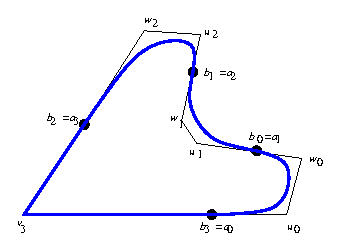
\includegraphics{potracelib-fig5}
  \]
  \caption{A closed curve consisting of 4 segments}\label{fig-curve}
\end{figure}

A curve in Potrace is a sequence of segments, such that the endpoint
of each segment coincides with the starting point of the next one. All
curves in Potrace are closed, and therefore the endpoint of the final
segment also coincides with the starting point of the first one.
Figure~\ref{fig-curve} shows an example of a curve consisting of 4
segments: 3 Bezier curve segments and 1 corner segment. For clarity,
the start- and endpoints of segments have been marked with dots
``$\bullet$''.

Curves are represented as values of type \verb!potrace_curve_t!,
which is defined as follows:

\begin{verbatim}
struct potrace_curve_s {
  int n;                    /* number of segments */
  int *tag;                 /* array of segment types */
  potrace_dpoint_t (*c)[3]; /* array of control points. */
};
typedef struct potrace_curve_s potrace_curve_t;
\end{verbatim}

Here $n\geq 1$ is the number of segments in the curve. For $i=0,\ldots,n-1$,
$\verb!tag[i]!$ is the type of the $i$-th segment, which is
\verb!POTRACE_CURVETO! for a Bezier curve segment and
\verb!POTRACE_CORNER! for a corner segment. $c$ is an array of size
$n\times 3$ that holds the control points of the curve segments in
the following manner:
\begin{itemize}
\item If the $i$-th segment is a Bezier curve segment, then
  $\verb!c[i][0]! = u$ and $\verb!c[i][1]! = w$ are the two control
  points of that segment, and $\verb!c[i][2]! = b$ is its endpoint.
\item If the $i$-th segment is a corner segment, then $\verb!c[i][0]!$
  is unused, $\verb!c[i][1]! = v$ is the vertex of the segment, and
  $\verb!c[i][2]! = b$ is its endpoint.
\end{itemize}

Note that, since the starting point $a$ of each segment coincides with
the endpoint $b$ of the preceding segment (and the starting point $a$
of the first segment coincides with the endpoint $b$ of the last
segment), there is no need to store the starting points $a$
explicitly. Also, note that regardless of the type of segment, the
endpoint of the $i$-th segment is $\verb!c[i][2]!$, and the starting point
of the $i$-th segment is $\verb!c[i ? i-1 : n-1][2]!$.

The curve from Figure~\ref{fig-curve} is therefore represented
by the following data:
\[\begin{array}{llll}
\verb!n = 4;!\\
\verb!tag[0] = POTRACE_CURVETO;!\\
\verb!c[0][0] = !u_0\verb!;!\quad\quad\quad
\verb!c[0][1] = !w_0\verb!;!\quad
\verb!c[0][2] = !b_0\verb! = !a_1\verb!;!\\
\verb!tag[1] = POTRACE_CURVETO;!\\
\verb!c[1][0] = !u_1\verb!;!\quad\quad\quad
\verb!c[1][1] = !w_1\verb!;!\quad
\verb!c[1][2] = !b_1\verb! = !a_2\verb!;!\\
\verb!tag[2] = POTRACE_CURVETO;!\\
\verb!c[2][0] = !u_2\verb!;!\quad\quad\quad
\verb!c[2][1] = !w_2\verb!;!\quad
\verb!c[2][2] = !b_2\verb! = !a_3\verb!;!\\
\verb!tag[3] = POTRACE_CORNER;!\\
\verb!c[3][0] = !{\it unused}\verb!;!\quad
\verb!c[3][1] = !v_3\verb!;!\quad
\verb!c[3][2] = !b_3\verb! = !a_0\verb!;!\\
\end{array}
\]

\subsubsection{Boundary decomposition of bitonal vector
  images}\label{sssec-boundary}

\begin{figure}
  \[\begin{array}{l@{\hspace{.25in}}l}
    (a) & (b) \\
    
\includegraphics{potracelib-fig1a}&
    
\includegraphics{potracelib-fig1b}
  \end{array}
  \]
  \caption{(a) A vector image. (b) Its boundary
    decomposition.}\label{fig-vector}
\end{figure}

In Potrace, a bitonal (i.e. black-and-white) vector image, as in
Figure~\ref{fig-vector}(a), is decomposed into a collection of closed
boundary curves, shown in blue and red and labeled $A$--$I$ in
Figure~\ref{fig-vector}(b).

We introduce some terminology. A closed curve is {\em simple} if it
does not intersect itself. Each simple closed curve, taken by itself,
divides the plane into two regions, called the {\em inside} and and
the {\em outside} of the curve. If $C_1$ and $C_2$ are simple closed
curves, we say that $C_1$ is {\em contained} in $C_2$, written $C_1 <
C_2$, if $C_1$ lies entirely within the inside of $C_2$. For example,
in Figure~\ref{fig-vector}(b), the curves $B$--$E$ are contained in
$A$, whereas $F$--$I$ are not.

In a decomposition of a vector image as in Figure~\ref{fig-vector}, we
say that a curve $C_1$ is a {\em child} of $C_2$ if $C_1 < C_2$ and
there exists no other curve $C_3$ between $C_1$ and $C_2$ (i.e., no
curve $C_3$ such that $C_1 < C_3 < C_2$). In this case, we also say
that $C_1$ is a {\em parent} of $C_2$. Since boundary curves do not
intersect, each curve has at most one parent.  Two curves are said to
be {\em siblings} if they are either both parentless, or else they
have a parent in common. Note that the ``child'' relation naturally
defines a tree structure on the set of curves (more precisely, it
defines a ``forest'', since there can be more than one root).

For example, in Figure~\ref{fig-vector}(b), the curve $A$ has no
parent, and has children $B$ and $E$. The curve $E$ has no children,
and the curve $B$ has children $C$ and $D$. $A$ and $F$ are siblings,
$B$ and $E$ are siblings, and $C$ and $D$ are siblings. The curves
from Figure~\ref{fig-vector}(b) form the following forest under the
``child'' relation:

\begin{verbatim}
                  A         F
                 / \        |
                B   E       G
               / \          |
              C   D         H
                            |
                            I
\end{verbatim}

We can assign each curve a {\em sign} by calling a curve {\em
  positive} if it encloses a ``foreground'' region, and {\em negative}
if it encloses a ``background'' region (or ``hole''). For example, in
Figure~\ref{fig-vector}(b), positive curves are shown in blue and
negative curves in red.

Since foreground and background regions alternate, it follows that the
sign of curves also alternates, i.e., parentless curves are always
positive, and all other curves have the opposite sign of their parent.
It follows that, in the tree structure, curves that appear at even
levels are positive and those that appear at odd levels are negative.
In particular, siblings share a common sign.

\subsubsection{Representation of vector images}\label{sssec-vector}

In Potrace, a vector image is represented as a linked collection of
zero or more structures of type \verb!potrace_path_t!, which is
defined as follows:

\begin{verbatim}
struct potrace_path_s {
  int area;                         /* enclosed area */
  int sign;                         /* '+' or '-' */
  potrace_curve_t curve;            /* vector data */

  struct potrace_path_s *next;      /* list structure */

  struct potrace_path_s *childlist; /* tree structure */
  struct potrace_path_s *sibling;   /* tree structure */

  struct potrace_privpath_s *priv;  /* private state */
};
typedef struct potrace_path_s potrace_path_t;
\end{verbatim}

Each such structure holds a single curve, and the structures are
linked to each other via the \verb!next!, \verb!childlist!, and
\verb!sibling! pointers.

\begin{itemize}

\item The \verb!sign! field holds the sign of the curve (\verb!'+'! or
  \verb!'-'! in ASCII).

\item The \verb!curve! field contains the curve's vector data as
  described in Section~\ref{sssec-curves}. Potrace additionally
  follows the convention that positive curves run counterclockwise and
  negative curves run clockwise; this facilitates rendering in
  environments (such as PostScript or PDF) that have a ``fill'' rule
  based on winding number.

\item The \verb!area! field gives the approximate magnitude of the
  area enclosed by the curve. (In fact, it is the precise integer area
  of the original untraced ``jaggy'' curve). Some clients use this
  information to improve interactive rendering speeds by ignoring very
  small areas in a first rendering pass. See also the description of
  the \verb!turdsize!  parameter in Section~\ref{ssec-parameters} below.
  
\item The \verb!priv!  field is used internally by Potrace, and is not
  accessible to applications.

\item The \verb!next! field is used to link all the curves of a given
  vector image into a linked list. Each member points to the next one
  via its \verb!next! field, and the last member of the list has
  \verb!next==NULL!.  The order of the elements of this list is
  unspecified, but is guaranteed to satisfy the following constraints:
  \begin{enumerate}\alphalabels
  \item outer curves appear before inner ones, so if $C_1 < C_2$, then
    $C_2$ always appears sometime before $C_1$ in the linked list, and
  \item each positive curve is immediately followed by all of its
    children.
  \end{enumerate}
  These two constraints make it easy for clients to render the image
  by simply processing the linked list in sequential order.
  Constraint (a) makes it possible to fill each curve with solid black
  or white color, allowing later curves to paint over parts of earlier
  ones.  Constraint (b) further allows a client to fill a positive
  curve, minus its negative children, in a single paint operation,
  leaving a ``hole'' for each of the negative children.

\item The \verb!childlist! and \verb!sibling! fields define a forest
  structure on the set of curves, which can be used independently of
  the linked list structure.  For each curve, \verb!childlist! is a
  pointer to its first child, or \verb!NULL! if there are no children.
  Also, \verb!sibling! is a pointer to the next sibling, or
  \verb!NULL!  if there are no further siblings.  The relative order
  of siblings is unspecified. The root node of the tree structure
  always coincides with the root node of the linked list structure.
\end{itemize}

An image consisting of zero curves is represented as a \verb!NULL! pointer.

\subsubsection{Intersecting curves}

While in the above discussion we have assumed a set of
non-intersecting curves, in practice it can happen that the curves
output by Potrace intersect slightly. Clients should therefore
carefully choose their rendering parameters (e.g., the non-zero
winding number rule is preferable to the odd winding number rule) to
avoid undesirable artifacts.

\subsubsection{Example}

The image from Figure~\ref{fig-vector} can be represented by the
pointer \verb!plist!, where {\tt A}--{\tt I} are structures
of type \verb!potrace_path_t!, as follows.  We do not show the
\verb!area! and \verb!curve! fields.
{\small
\begin{verbatim}
 potrace_path_t *plist = &A;

 A.sign = '+';       B.sign = '-';       E.sign = '-';
 A.next = &B;        B.next = &E;        E.next = &C;
 A.childlist = &B;   B.childlist = &C;   E.childlist = NULL;
 A.sibling = &F;     B.sibling = &E;     E.sibling = NULL;

 C.sign = '+';       D.sign = '+';       F.sign = '+';
 C.next = &D;        D.next = &F;        F.next = &G;
 C.childlist = NULL; D.childlist = NULL; F.childlist = &G;
 C.sibling = &D;     D.sibling = NULL;   F.sibling = NULL;

 G.sign = '-';       H.sign = '+';       I.sign = '-';
 G.next = &H;        H.next = &I;        I.next = NULL;
 G.childlist = &H;   H.childlist = &I;   I.childlist = NULL;
 G.sibling = NULL;   H.sibling = NULL;   I.sibling = NULL;
\end{verbatim}
}

\subsection{Tracing parameters}\label{ssec-parameters}

The tracing operation of Potrace is controlled by a small number of
parameters. The parameter structure is defined in potracelib.h as:

\begin{verbatim}
struct potrace_param_s {
  int turdsize;        
  int turnpolicy;      
  double alphamax;     
  int opticurve;       
  double opttolerance; 
  potrace_progress_t progress; 
};
typedef struct potrace_param_s potrace_param_t;
\end{verbatim}

For most practical purposes, the default parameters give excellent
results. The function \verb!potrace_param_default()! (see
Section~\ref{5c}) returns the set of default parameters. Applications
must always start from these default parameters before changing any
parameters. This will increase backward compatibility in case
additional parameters are added in the future.

\subsubsection{Turdsize}

\begin{figure}
\[\begin{array}{l@{\hspace{.5in}}l}
  \textrm{\rm Before:} & \textrm{\rm After:}\\
  
\includegraphics{potracelib-fig6a}&
  
\includegraphics{potracelib-fig6b}
\end{array}
\]
\caption{Despeckling with turdsize=3.}\label{fig-turdsize}
\end{figure}

The \verb!turdsize! parameter can be used to ``despeckle'' the bitmap
to be traced, by removing all curves whose enclosed area is below the
given threshold. Figure~\ref{fig-turdsize} shows the result of
applying turdsize=3 to a bitmap. The current default for the turdsize
parameter is 2; its useful range is from 0 to infinity.

\subsubsection{Turnpolicy}

\begin{figure}
\[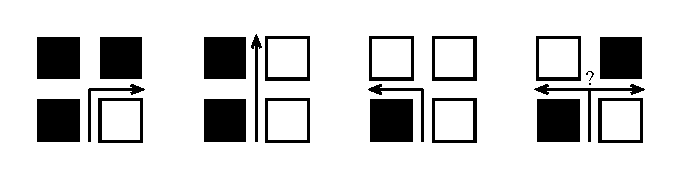
\includegraphics{potracelib-fig8}\]
\caption{Path decomposition}\label{fig-turns}
\end{figure}

The turnpolicy parameter determines how to resolve ambiguities during
decomposition of bitmaps into paths. The ambiguity arises in the last
situation shown in Figure~\ref{fig-turns}. The possible choices for
the \verb!turnpolicy! parameter are:
\begin{itemize}
\item \verb!POTRACE_TURNPOLICY_BLACK!: prefers to connect black
  (foreground) components.
\item \verb!POTRACE_TURNPOLICY_WHITE!: prefers to connect white
  (background) components.
\item \verb!POTRACE_TURNPOLICY_LEFT!: always take a left turn.
\item \verb!POTRACE_TURNPOLICY_RIGHT!: always take a right turn.
\item \verb!POTRACE_TURNPOLICY_MINORITY!: prefers to connect the color
  (black or white) that occurs least frequently in a local
  neighborhood of the current position.
\item \verb!POTRACE_TURNPOLICY_MAJORITY!: prefers to connect the color
  (black or white) that occurs most frequently in a local neighborhood
  of the current position.
\item \verb!POTRACE_TURNPOLICY_RANDOM!: choose pseudo-randomly.
\end{itemize}

The current default policy is \verb!POTRACE_TURNPOLICY_MINORITY!, which tends
to keep visual lines connected.

\subsubsection{Alphamax}

\begin{figure}
\[\begin{array}{ccccc}

\includegraphics{potracelib-fig7-00}&

\includegraphics{potracelib-fig7-06}&

\includegraphics{potracelib-fig7-10}&

\includegraphics{potracelib-fig7-12}&

\includegraphics{potracelib-fig7-13}\\
\alpha_{max}=0.0&
\alpha_{max}=0.6&
\alpha_{max}=1.0&
\alpha_{max}=1.2&
\alpha_{max}=1.3
\end{array}
\]
\caption{The alphamax parameter}\label{fig-alphamax}
\end{figure}

The \verb!alphamax! parameter is a threshold for the detection of
corners. It controls the smoothness of the traced curve, as shown in
Figure~\ref{fig-alphamax}. The current default is 1.0.  The useful range of
this parameter is from 0.0 (polygon) to 1.3334 (no corners).

\subsubsection{Opticurve and opttolerance}

The \verb!opticurve! parameter is a boolean flag that controls whether
Potrace will attempt to ``simplify'' the final curve by reducing the
number of Bezier curve segments. Opticurve=1 turns on optimization,
and opticurve=0 turns it off. The current default is on. 

The \verb!opttolerance! parameter defines the amount of error allowed
in this simplification. The current default is 0.2. Larger values tend to
decrease the number of segments, at the expense of less accuracy.  The
useful range is from 0 to infinity, although in practice one would
hardly choose values greater than 1 or so. For most purposes, the
default value is a good tradeoff between space and accuracy.

\subsubsection{Progress reporting}

Since tracing a large bitmap can be time consuming, Potrace has the
option of reporting progress to the calling application. This is
typically used in interactive applications to implement a progress
bar. Progress reporting is controlled by the \verb!progress!
parameter, which is a structure of type \verb!potrace_progress_t!,
defined as follows:

\begin{verbatim}
struct potrace_progress_s {
  void (*callback)(double progress, void *privdata);
  void *data;      
  double min, max; 
  double epsilon;      
};
typedef struct potrace_progress_s potrace_progress_t;
\end{verbatim}

If \verb!callback! is not NULL, then progress reporting is enabled.
In this case, \verb!callback! is the address of a function to be
called for progress reports, and \verb!data! is a pointer to that
function's private data.  Progress reports take the form of a function
call \verb!callback(d, data)!, where \verb!d! is a number representing
the amount of relative progress in the range
\verb!min!\ldots\verb!max!. 

The parameter \verb!epsilon! is a hint that tells Potrace what amount of
progress the application considers ``too small to report''. Whenever
convenient, Potrace will feel free to suppress progress reports if the
increment since the previous report has been less than \verb!epsilon!.  As
a special case, if $\verb!epsilon!=0$, then the maximal number of progress
reports are sent. In any case, the application should handle progress
reports very efficiently, as there may be a large number of reports. 

The defaults are $\verb!callback!=\textrm{NULL}$,
$\verb!data!=\textrm{NULL}$, $\verb!min!=0.0$, $\verb!max!=1.0$, and
$\verb!epsilon!=0$.

\subsection{Potrace state}\label{4}

A Potrace state holds the result of a tracing operation. It is
defined as follows:

\begin{verbatim}
struct potrace_state_s {
  int status;
  potrace_path_t *plist;            /* vector data */

  struct potrace_privstate_s *priv; /* private state */
};
typedef struct potrace_state_s potrace_state_t;
\end{verbatim}

The fields are as follows:
\begin{itemize}
\item The \verb!status! field is either \verb!POTRACE_STATUS_OK!, to
  indicate that the tracing operation was successful, or
  \verb!POTRACE_STATUS_INCOMPLETE!, to indicate that it was
  unsuccessful.
\item In the event of success, \verb!plist! points to the
  representation of the bitonal traced vector image as described in
  Section~\ref{sssec-vector}.  In the event of failure, \verb!plist!
  points to a data structure whose properties are undefined, except
  that the Potrace state can still be freed with \verb!potrace_state_free()!.
\item The \verb!priv! field is used internally by Potrace, and is not
  accessible by applications.
\end{itemize}

\section{API functions}\label{5}

There is no global or static state in potracelib; all API functions
are reentrant and thread-safe.

\subsection{potrace\_trace}\label{5a}

{\small
\begin{verbatim}
potrace_state_t *potrace_trace(const potrace_param_t *param,
                               const potrace_bitmap_t *bm);
\end{verbatim}
}

\noindent Inputs: 
\begin{itemize}
\item \verb!bm!: a bitmap (see Section~\ref{ssec-bitmap}).
\item \verb!param!: a set of tracing parameters (see
  Section~\ref{ssec-parameters}).
\end{itemize}

\noindent Output:
\begin{itemize}
\item a Potrace state (see Section~\ref{4}). 
\end{itemize}

This function attempts to trace the given bitmap using the given
tracing parameters. In the event of success, it returns a valid
Potrace state with the \verb!status! field set to
\verb!POTRACE_STATUS_OK!.  In the event of failure, it sets
\verb!errno! to an error number, and either returns \verb!NULL!, or
else it returns an incomplete Potrace state, which by definition has
the status field set to \verb!POTRACE_STATUS_INCOMPLETE!. Any Potrace
state returned by \verb!potrace_trace()! (whether it is valid or
invalid) can be freed using the \verb!potrace_state_free()! function
below.

\subsection{potrace\_state\_free}\label{5b}

\begin{verbatim}
void potrace_state_free(potrace_state_t *st);
\end{verbatim}

\noindent Input:
\begin{itemize}
\item \verb!st!: a Potrace state previously returned by
  \verb!potrace_trace()!.
\end{itemize}

This function frees the memory and other resources (if any) associated
with the Potrace state.

\subsection{potrace\_param\_default}\label{5c}

\begin{verbatim}
potrace_param_t *potrace_param_default();
\end{verbatim}

\noindent Output:
\begin{itemize}
\item a set of tracing parameters (see Section~\ref{ssec-parameters}). 
\end{itemize}

This function returns a fresh set of tracing parameters, initialized
to defaults.  Applications must always use this function to create an
object of type \verb!potrace_param_t!, and they must always start from
the default parameters before modifying any parameters.  This will
help increase backward compatibility when additional parameters are
added in the future. The parameter set returned by this function can
later be freed by \verb!potrace_param_free()!.

\subsection{potrace\_param\_free()}\label{5d}

\begin{verbatim}
void potrace_param_free(potrace_param_t *p);
\end{verbatim}

\noindent Input:
\begin{itemize}
\item tracing parameters previously returned by
  \verb!potrace_param_default()!.
\end{itemize}

This function frees the memory occupied by a set of tracing parameters
as returned by \verb!potrace_param_default()!. Only the fields
initialized by Potrace are freed, not any fields set by the
application itself (such as \verb!progress.data!).

\subsection{potrace\_version()}\label{5e}

\begin{verbatim}
const char *potrace_version();
\end{verbatim}

This function returns a static human-readable text string identifying
this version of potracelib.

\end{document}
